\section{Evaluation Comparison}\label{sec:result_comparison}
In the final evaluation step we take a broader look on the overall performance of context enrichment. For that, we combined the results from each dataset. This has the advantage of reducing the sensibility to a particular dataset which is desirable for unbiased conclusions. 

Based on our initial hypothesis which motivates adding context to ontology validation we formulated a couple of questions that were answered next:
\paragraph{Which Context Enrichment Method performed best in general?}
\begingroup
\renewcommand{\arraystretch}{1.5}
\begin{table}
	\begin{tabularx}{\textwidth}{l c*{3}{Y}}
		\toprule
		Method & Precision & Recall & F-Measure \\
		\midrule
		 Embedded Context & 0.797 & 0.921 & 0.854 \\
		 Neighbouring Nodes & 0.787 & 0.887 & 0.834 \\
		 External Source & 0.729 & 0.899 & 0.805 \\
		 None & 0.674 & 0.910 & 0.775 \\
		\bottomrule
	\end{tabularx}
	\caption{Aggregated results of all datasets~(ranked by F-Measure)}
	\label{table:bench_p_r_f_combined}
\end{table}
\endgroup

\begin{figure}
	 \centering
	 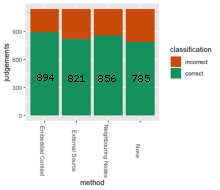
\includegraphics[width=0.75\textwidth]{plots/comparison/barplot_all_judgements}
	 \caption{Combined accuracy of crowdsourcing methods}\label{fig:results_accuracy_combined}
\end{figure}

Lorem ipsum dolor sit amet, consectetur adipisicing elit, sed do eiusmod tempor incididunt ut labore et dolore magna aliqua. Ut enim ad minim veniam, quis nostrud exercitation ullamco laboris nisi ut aliquip ex ea commodo consequat. Duis aute irure dolor in reprehenderit in voluptate velit esse cillum dolore eu fugiat nulla pariatur. Excepteur sint occaecat cupidatat non proident, sunt in culpa qui officia deserunt mollit anim id est laborum.

\paragraph{Did the crowd perform better with context?}
% No chart needed, the charts from the question above can be used %
Lorem ipsum dolor sit amet, consectetur adipisicing elit, sed do eiusmod tempor incididunt ut labore et dolore magna aliqua. Ut enim ad minim veniam, quis nostrud exercitation ullamco laboris nisi ut aliquip ex ea commodo consequat. Duis aute irure dolor in reprehenderit in voluptate velit esse cillum dolore eu fugiat nulla pariatur. Excepteur sint occaecat cupidatat non proident, sunt in culpa qui officia deserunt mollit anim id est laborum.

\paragraph{For which concepts were the crowd wrong?}
\begingroup
\renewcommand{\arraystretch}{1.5}
\begin{table}
	\begin{tabularx}{\textwidth}{l c*{4}{Y}}
		\toprule
		\multirow{2}{*}{\emph{Concept}} & \multicolumn{4}{c}{\emph{Methods}} & \emph{Accuracy}\\
		\cmidrule(lr){2-5} \cmidrule(lr){6-6} 
		 & EC & NN & ES & NONE & Total\\
		\midrule
		sceptic & 0/5 & 0/5 & 0/5 & 0/5 & 0/20 \\
		greenhouse & 0/5 & 1/5 & 0/5 & 0/5 & 1/20 \\
		pipeline & 0/5 & 0/5 & 1/5 & 0/5 & 1/20 \\
		consensus & 2/5 & 0/5 & 0/5 & 0/5 & 2/20 \\
		denier & 2/5 & 0/5 & 0/5 & 0/5 & 2/20 \\
		production & 1/5 & 1/5 & 0/5 & 0/5 & 2/20 \\
		\bottomrule
	\end{tabularx}
	\caption{Concepts where most crowd workers had problems~(EC=Embedded Context, NN=Neighbouring Nodes, ES=External Source, NONE=No Context)}
	\label{table:bench_p_r_f_combined}
\end{table}
\endgroup

Lorem ipsum dolor sit amet, consectetur adipisicing elit, sed do eiusmod tempor incididunt ut labore et dolore magna aliqua. Ut enim ad minim veniam, quis nostrud exercitation ullamco laboris nisi ut aliquip ex ea commodo consequat. Duis aute irure dolor in reprehenderit in voluptate velit esse cillum dolore eu fugiat nulla pariatur. Excepteur sint occaecat cupidatat non proident, sunt in culpa qui officia deserunt mollit anim id est laborum.

\paragraph{What other observations were found?}
Lorem ipsum dolor sit amet, consectetur adipisicing elit, sed do eiusmod tempor incididunt ut labore et dolore magna aliqua. Ut enim ad minim veniam, quis nostrud exercitation ullamco laboris nisi ut aliquip ex ea commodo consequat. Duis aute irure dolor in reprehenderit in voluptate velit esse cillum dolore eu fugiat nulla pariatur. Excepteur sint occaecat cupidatat non proident, sunt in culpa qui officia deserunt mollit anim id est laborum.